\documentclass[a4paper,11pt]{article}
\input{/home/tof/Documents/Cozy/latex-include/preambule_lua.tex}
\newcommand{\showprof}{show them}  % comment this line if you don't want to see todo environment
\fancyhead[L]{Évolution de la température - type construit de données}
\newdate{madate}{10}{09}{2020}
\fancyhead[R]{Première - NSI} %\today
\fancyfoot[L]{~\\Christophe Viroulaud}
\fancyfoot[C]{\textbf{Page \thepage}}
\fancyfoot[R]{\includegraphics[width=2cm,align=t]{/home/tof/Documents/Cozy/latex-include/cc.png}}
\usepackage{tikz}
\begin{document}
\begin{Form}
%DODO tab en paramètre d'une fonction = on envoie une référence du tab: si tab est grand Python ne va pas tt recopier (trop de place mémoire); donc attention aux modifs de tab
\begin{commentprof}
Mettre fichier tuple.zip sur site avant le cours
\end{commentprof}
\section{Problématique}
Dans le cadre d'une exposition sur l'évolution du climat, le professeur de SVT nous demande de réaliser un programme pour manipuler les données de température moyenne en France. Ces valeurs sont aisément accessibles sur le web.
\begin{figure}[!h]
\centering
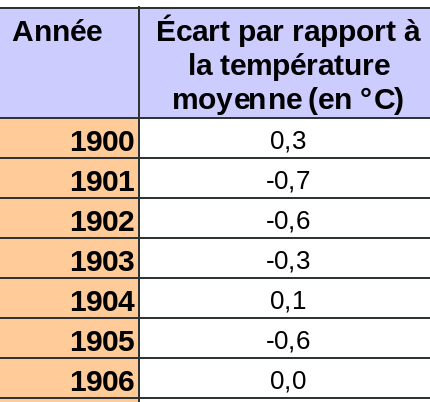
\includegraphics[width=5cm]{ressources/extrait.png}
\captionof{figure}{Anomalie de la température moyenne annuelle de l'air par rapport à la moyenne de référence. Le zéro correspond à la moyenne de l'indicateur sur la période 1961-1990, soit 11,8 °C}
\label{extrait}
\end{figure}

Il est possible de créer une variable pour chaque année, mais cela va être rapidement fastidieux.
\begin{code}[!h]
\begin{lstlisting}
annee1900 = 0.3
annee1901 = -0.7
...
\end{lstlisting}
\captionof{code}{Une variable par année}
\label{moncode}
\end{code}
\begin{center}
\shadowbox{\parbox{15cm}{\centering Comment stocker les données dans le programme pour les manipuler facilement?}}
\end{center}
\section{Les tuples}
\subsection{Présentation}
Un \emph{tuple} est une séquence \textbf{ordonnée} de plusieurs éléments. En mathématiques on parle de \emph{p-uplet}.
\begin{commentprof}
un quadruplet = 4 éléments; on peut le voir comme un tableau fixe
\end{commentprof}
\begin{code}[!h]
\begin{lstlisting}
mon_tuple = (8, 5, 3, 9, 1, 0, 2)
\end{lstlisting}
\captionof{code}{Créer un tuple en Python}
\label{tuple1}
\end{code}
\subsection{Accéder à un élément}
On ne peut modifier un tuple: on dit qu'il est \emph{immuable} ou \emph{non mutable}. Par contre il est possible d'accéder aux éléments individuellement.
\begin{code}[!h]
\begin{lstlisting}
>>> mon_tuple[0]
>>> 8
\end{lstlisting}
\captionof{code}{Accéder à l'élément de rang 0}
\label{acces}
\end{code}

Le code \ref{acces} renvoie la première valeur du tuple. \textbf{L'indexation commence à 0.}\\
Chaque élément est accessible en \emph{temps constant} même si le tuple est très important.
\begin{figure}[!h]
\centering
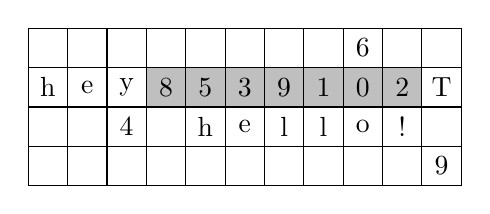
\begin{tikzpicture}[scale=0.5]
\fill[gray!50] (3,2) rectangle (10,3);
\draw (0,0) grid (11,4);

\draw (0.5,2.5) node{h};
\draw (1.5,2.5) node{e};
\draw (2.5,2.5) node{y};
\draw (10.5,2.5) node{T};

\draw (4.5,1.5) node{h};
\draw (5.5,1.5) node{e};
\draw (6.5,1.5) node{l};
\draw (7.5,1.5) node{l};
\draw (8.5,1.5) node{o};
\draw (9.5,1.5) node{!};

\draw (10.5,0.5) node{9};
\draw (8.5,3.5) node{6};
\draw (2.5,1.5) node{4};

\foreach \x/\y in {3/8,4/5,5/3,6/9,7/1,8/0,9/2}
{\draw (\x+0.5,2.5) node{\y};}
\end{tikzpicture}
\captionof{figure}{Le tuple est enregistré dans un espace libre}
\end{figure}
\subsection{Utiliser le tuple}
Le tuple ci-après contient les anomalies de températures de 1900 à 2017.
\lstinputlisting[firstline=17,lastline=28, xleftmargin=2em,
	xrightmargin=2em]{"scripts/temperature-france.py"}
\begin{activite}
\begin{enumerate}
\item Récupérer le code \emph{temperature.py} sur le site \url{https://cviroulaud.github.io}
\item Afficher l'anomalie de température pour l'année 1910.
\item Écrire un programme qui demande une année à l'utilisateur et affiche l'anomalie correspondante.
\item Tester le code \ref{graphe} qui utilise la bibliothèque \emph{pyplot}. Prendre le temps de comprendre la ligne 3.
\end{enumerate}
\begin{center}
\lstinputlisting[firstline=30,lastline=34]{"scripts/temperature-france.py"}
\captionof{code}{Première utilisation de la bibliothèque matplotlib.pyplot}
\label{graphe}
\end{center}
\end{activite}
\begin{figure}[!h]
\centering
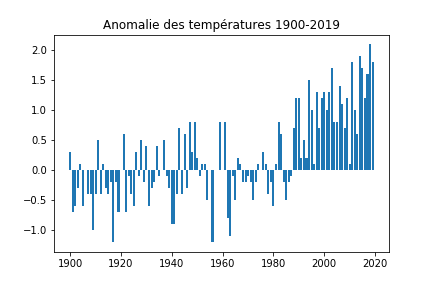
\includegraphics[width=8cm]{ressources/temp.png}
\captionof{figure}{Anomalie des températures 1900 - 2017}
\label{resgraphe}
\end{figure}
\section{Les tableaux}
\subsection{Présentation}
Les tuples sont très utiles mais restent limités: on ne peut pas les modifier. Or si nous voulons rajouter les années 2018 et 2019 dans nos données, nous sommes obligés de créer un nouveau tuple. Ce n'est guère satisfaisant.\\
Un deuxième type de structure semble alors plus adapté: \emph{les tableaux}.
\begin{code}[!h]
\begin{lstlisting}
mon_tableau = [8, 5, 3, 9, 1, 0, 2]
\end{lstlisting}
\captionof{code}{Créer un tableau}
\label{tableau}
\end{code}

\textbf{À savoir:} En Python, ces structures portent le nom \emph{list}. Cependant cela peut prêter confusion avec un autre type de construction que nous verrons l'année prochaine.
\subsection{Accéder à un élément}
La syntaxe est la même que pour les tuples.
\begin{code}[!h]
\begin{lstlisting}
>>> mon_tableau[0]
>>> 8
\end{lstlisting}
\captionof{code}{Accéder au premier élément}
\label{accestab}
\end{code}

Il est également possible de modifier un élément.
\begin{center}
\begin{lstlisting}
mon_tableau[2] = 19
\end{lstlisting}
\captionof{code}{Modification du troisième élément}
\label{modif}
\end{center}
\subsection{Ajouter un élément}
Les tableaux sont \emph{mutables}. Il est possible de modifier leur contenu, ajouter voire supprimer un élément.
\begin{code}[!h]
\begin{lstlisting}
mon_tableau.append(12)
\end{lstlisting}
\captionof{code}{Ajouter un élément en fin de liste}
\label{ajout}
\end{code}
\subsection{Pour aller plus loin}
Il existe de nombreuses autres méthodes pour manipuler les tableaux. La documentation Python présente ces outils.
\begin{center}
\url{https://docs.python.org/fr/3/tutorial/datastructures.html}
\end{center}
\subsection{Utiliser le tableau}
En 2018 l'anomalie de température était de +2.1. En 2019, elle s'élevait à +1.8.
\begin{activite}
\begin{enumerate}
\item Modifier le programme précédent pour qu'il utilise un tableau au lieu d'un tuple.
\item Ajouter les anomalies de 2018 et 2019 à l'aide de la méthode \emph{append}.
\item Réaliser la représentation graphique des anomalies.
\end{enumerate}
\end{activite}
\end{Form}
\end{document}